\documentclass[a4paper, 12pt]{article}
\usepackage{titling}
\usepackage{array}
\usepackage{booktabs}
\usepackage{enumitem}
\usepackage{graphicx}
\usepackage{hyperref}
\usepackage{amssymb}
%\usepackage{mathtools}
\usepackage{listings}
\usepackage{amsmath}
\usepackage{color} %red, green, blue, yellow, cyan, magenta, black, white
\setlength{\heavyrulewidth}{1.5pt}
\setlength{\abovetopsep}{4pt}
\setlength{\parindent}{0pt}
\graphicspath{{.}}
\usepackage{float}
\usepackage[margin=1in]{geometry}
\definecolor{mygreen}{RGB}{28,172,0} % color values Red, Green, Blue
\definecolor{mylilas}{RGB}{170,55,241}
% Must be after geometry
\usepackage{fancyhdr}
\pagestyle{fancy}
\fancyhf{}
\rhead{NN Homework 9}
\lhead{P.Lukin, E. Ovchinnikova}
\cfoot{\thepage}

\setlength{\droptitle}{-5em}

\title{Neural Networks  \\
				- Homework 9 -}
\author{Petr Lukin, Evgeniya Ovchinnikova}
\date{Lecture date: 28 November 2016}

\begin{document}

%-------------------------------------------------------------------------------
\lstset{language=Matlab,%
    %basicstyle=\color{red},
    breaklines=true,%
    morekeywords={matlab2tikz},
    keywordstyle=\color{blue},%
    morekeywords=[2]{1}, keywordstyle=[2]{\color{black}},
    identifierstyle=\color{black},%
    stringstyle=\color{mylilas},
    commentstyle=\color{mygreen},%
    showstringspaces=false,%without this there will be a symbol in the places where there is a space
    numbers=left,%
    numberstyle={\tiny \color{black}},% size of the numbers
    numbersep=9pt, % this defines how far the numbers are from the text
    emph=[1]{break},emphstyle=[1]\color{red}, %some words to emphasise
    emph=[2]{end,function}, emphstyle=[1]\color{blue},
}

%-------------------------------------------------------------------------------

\maketitle

\section{Mind map}
\begin{figure}[h]
  \centering
  \caption{Mind map. Chapter 15 from Haykin's book. A zoomed version is attached as RecurrentNetworks.png}
  \includegraphics[width=1.0\textwidth]{RecurrentNetworks}
\end{figure}

\newpage
\section{Exercises}

Train an ESN:

Acquaint yourselves with the MATLAB based Reservoir Computing Toolbox v2.0

(RCT) or with Python version of RCT or use PGPs own ESN generic MATLAB.

implementation (see folder Echo State Networks (Part1 + Part2)).

Using one of these tools suite do the following:
\begin{itemize}
\item Sample the function $\cos(x)$ function for ten full cycles with 20 data points per cycle;
\item get a data vector;
\item choose one supported off-line training method (for analog neurons);
\item train an ESN on these (no inputs $=>$ free runtime);
\item after training run the ESN for a long time such that the output of the ESN is;
\item significantly different from the original $\cos()$ function;
\item now think: why can this happen?
\end{itemize}

\section{Solution}

Reservoir computing Matlab toolbox by Herbert Jaege was used in this assignment. ESN will be used to model $\cos$ over 10 periods. Training data is $\cos(x)$ where $x \in~[0,10\pi]$ with step $\pi/20$, that makes 201 datapoints. The function looks like this:


\begin{center}
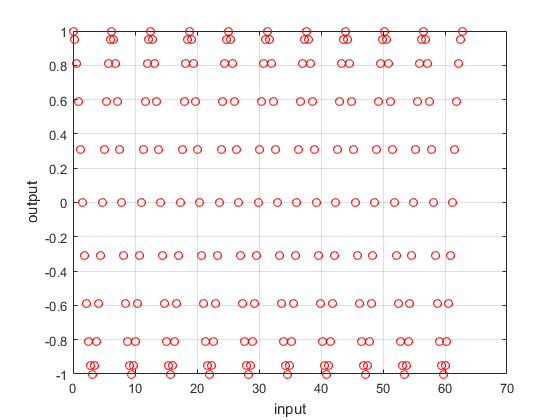
\includegraphics[scale=0.6]{traindata.png}
\end{center}

Training data is also $\cos(x)$ function on the same interval,but step size is smaller that gives 629 datapoints.

\begin{center}
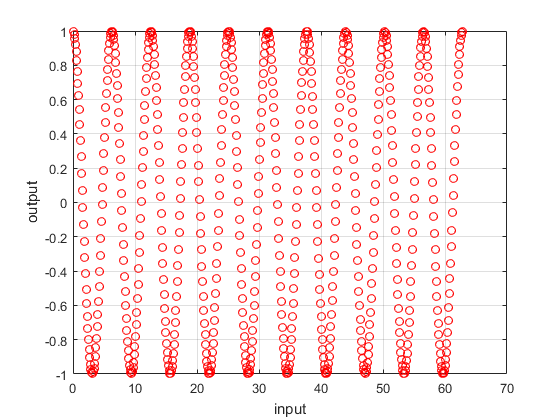
\includegraphics[scale=0.6]{testdata.png}
\end{center}


ESN were trained on the training set, with off line learning method and plain or leaky type. 

First test: 100 internal nodes plain vs leaky.

\begin{center}
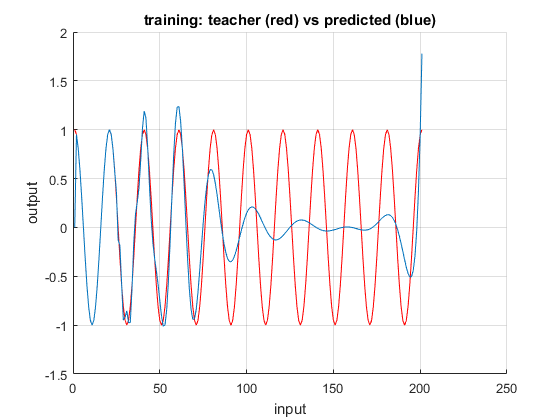
\includegraphics[scale=0.6]{100plain.png}

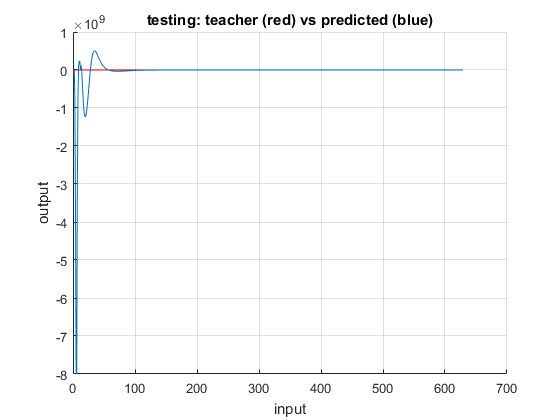
\includegraphics[scale=0.6]{100plaint.png}


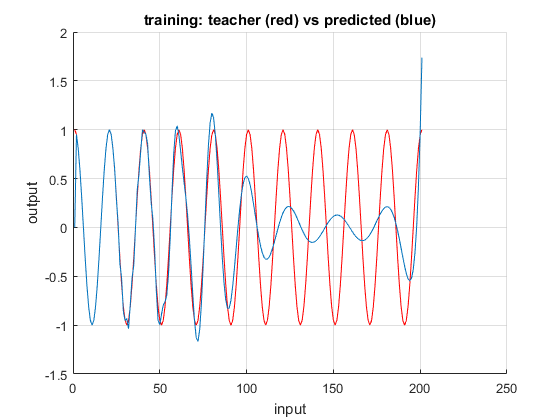
\includegraphics[scale=0.6]{100leaky.png}

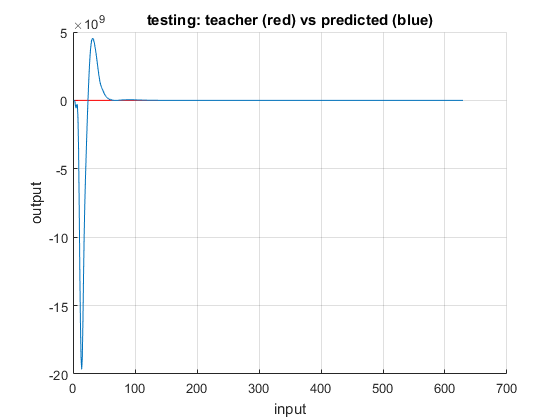
\includegraphics[scale=0.6]{100leakyt.png}
\end{center}

Using only 100 internal neurons, performance of the ESN is really low. However, Leaky network shows better results. Both failed in predicting data with other time sequence.


Second test: 500 internal nodes plain vs leaky.

\begin{center}
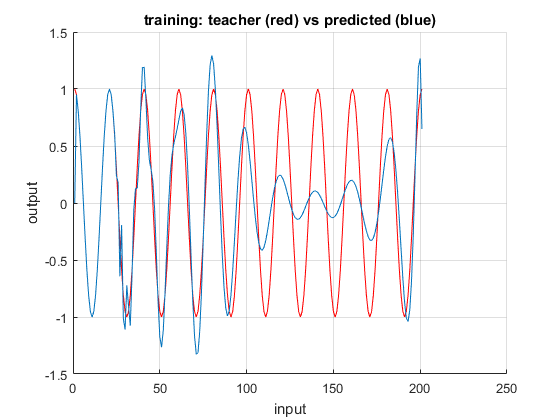
\includegraphics[scale=0.6]{500plain.png}

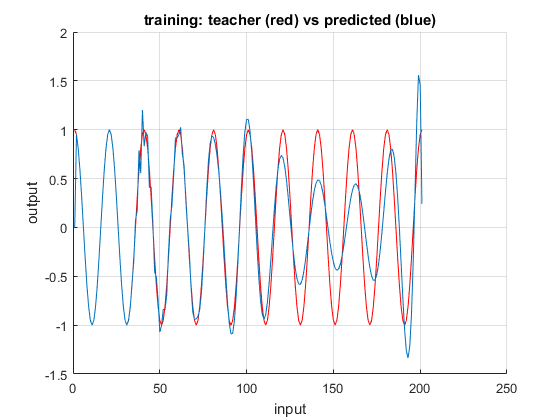
\includegraphics[scale=0.6]{500leaky.png}
\end{center}

With 500 internal neurons, performance of the ESN is better, but still unsatisfying. Both failed in predicting data with other time sequence again.


Third test: 5000 internal nodes plain vs leaky.

\begin{center}
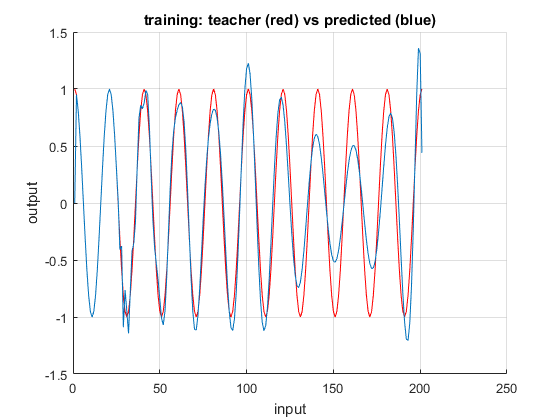
\includegraphics[scale=0.6]{5000plain.png}

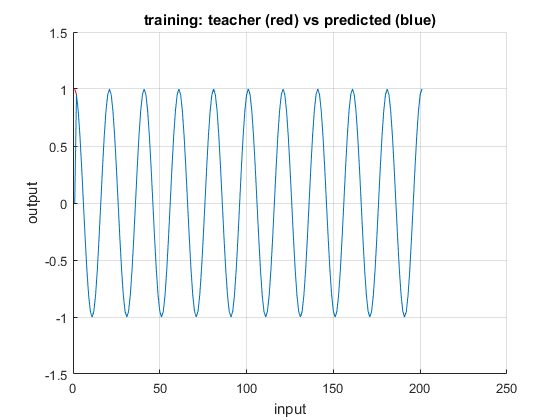
\includegraphics[scale=0.6]{5000leaky.png}
\end{center}

With 5000 internal neurons, plain ESN still doing bad, when Leaky ESN shows good precision. But, other timeseries still can not be predicted:

\begin{center}
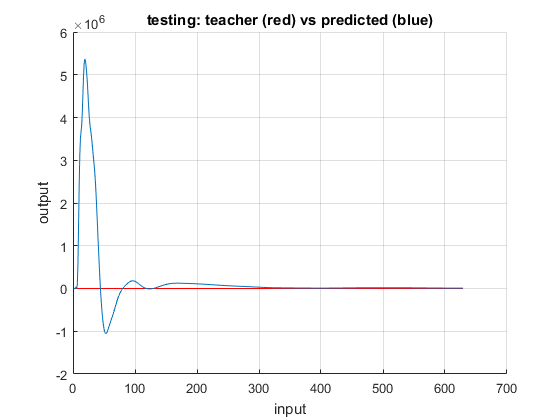
\includegraphics[scale=0.6]{5000lt.png}
\end{center}

If we increase number of testing data, we still will not obtain better prediction. This happens because ESN is strongly dependent on training dataset. Inner weights of the network are trained based on time series data. So, the ESN can only model data with similar time input.



\end{document}
